\documentclass[12pt]{beamer}
\usetheme{Pittsburgh}
\usepackage[spanish]{babel}
\usepackage{times}
\usepackage[T1]{fontenc}
\usepackage[utf8]{inputenc}
\usepackage{graphicx}
\usepackage{tikz}
\usepackage{listings}

%\usepackage{pgfpages}
%\pgfpagesuselayout{4 on 1}[a4paper,border shrink=5mm]

\renewcommand\shorthandsspanish{}
\noextrasspanish

\title{Curso de Matlab.  Nivel Básico}
\author{Guillem Borrell i Nogueras}

\begin{document}

\lstset{language=Matlab,
  backgroundcolor=\color{black!10},
  numbers=left,
  basicstyle=\small\ttfamily,
  keywordstyle=\color{blue},
  extendedchars=true,
  inputencoding=utf8,
  showspaces=false}

\begin{frame}
  \titlepage
\end{frame}

\begin{frame}
  \frametitle{Antes de empezar}
  \begin{itemize}
  \item Guillem Borrell i Nogueras.
  \item  \url{http://iimyo.forja.rediris.es/}
    \begin{itemize}
      \item Introducción Informal a Matlab y Octave
      \item Matemáticas en Ingeniería con Matlab y Octave
      \item Transparencias y ejercicios de este curso
      \item Material de otros cursos
    \end{itemize}
  \end{itemize}
\end{frame}

\begin{large}

  \begin{frame}
    \frametitle{Funcionamiento}
    \begin{itemize}
    \item Visitar la página del curso
    \item Descargarse la hoja de ejercicios
    \item Parar el vídeo para intentar el ejercicio antes que se de
      la solución.
    \end{itemize}
  \end{frame}

\begin{frame}
\frametitle{Recordad...}
\begin{center}
Ningún lenguaje se aprende por osmosis
\end{center}
\end{frame}

\begin{frame}
  \frametitle{¿Qué es Matlab?}
  \begin{itemize}
    \item{Un lenguaje de programación}
    \item{Un lenguaje de programación \emph{interpretado}}
    \item{Un lenguaje de programación \emph{interactivo}}
  \end{itemize}
  \begin{center}
    \textbf{Usar Matlab == Programar en Matlab}
  \end{center}
\end{frame}

\begin{frame}
  \frametitle{¿Qué no es Matlab}
  \begin{itemize}
    \item Una hoja de cálculo
    \item Un programa de cálculo simbólico.  Matlab puede hacer
      $\int_0^1 erf(x)\ dx = 0.486$ pero no 
      $\int erf(x)\ dx = x\ erf(x)+\frac{e^{-x^2}}{\sqrt{\pi}}$
    \item La solución a todos nuestros problemas.
  \end{itemize}
\end{frame}


\defverbatim[colored]\testcode{
  \begin{lstlisting}
    >>
  \end{lstlisting}
}

\begin{frame}
  \frametitle{¿Qué significa interpretado?}
  \begin{itemize}
    \item Un intérprete es un programa.
    \item Es como un actor que hace todo lo que le dice un
      \emph{guión}
    \item Muy parecido a la una calculadora.
    \item Es interactivo.
  \end{itemize}
  \testcode
  Os presento a la consola de Matlab
\end{frame}

\begin{frame}
\frametitle{Algunas mentiras}
\begin{itemize}
  \item Para ser ingeniero aeronáutico no es necesario saber
    programar.
  \item Programar es difícil.
  \item Programar \emph{bien} es fácil.
  \item Los ingenieros programan bien
  \item En la vida basta un lenguaje de programación mientras se
    domine.
\end{itemize}
\end{frame}

\begin{frame}
  \frametitle{Un autoengaño}
  \begin{LARGE}
  \begin{center}
    Si en la escuela sólo me dan seis créditos de informática es
    porque no es importante.
  \end{center}
  \end{LARGE}
\end{frame}

\begin{frame}
  \begin{LARGE}
  \begin{center}
    En Arquitectura nadie enseña Autocad.
  \end{center}
  \end{LARGE}
\end{frame}

\begin{frame}
\frametitle{Problema:}
Representar I(y), la integral de la función de Bessel

\[ I(y)=\int_0^y J_{2.5}(x)\ dx \]

con $y \in [1,5]$

\begin{itemize}
\item ¿Cómo se haría en Fortran?
\item ¿Cómo se haría en Excel?
\end{itemize}
\end{frame}

\defverbatim[colored]\testcode{
\begin{lstlisting}
x=linspace(1,5,100);
intbessel=@(y) quad(@(x) besselj(2.5,x),0,y);
for i=1:100
  z(i)=intbessel(x(i));
end
plot(x,z);
\end{lstlisting}
}

\begin{frame}
\frametitle{En Matlab son 6 líneas}
\testcode
No os preocupéis si no entendéis nada.  Esto es Matlab avanzado.
\end{frame}

\begin{frame}
\frametitle{El resultado}
  \begin{figure}[h]
    \centering{}
    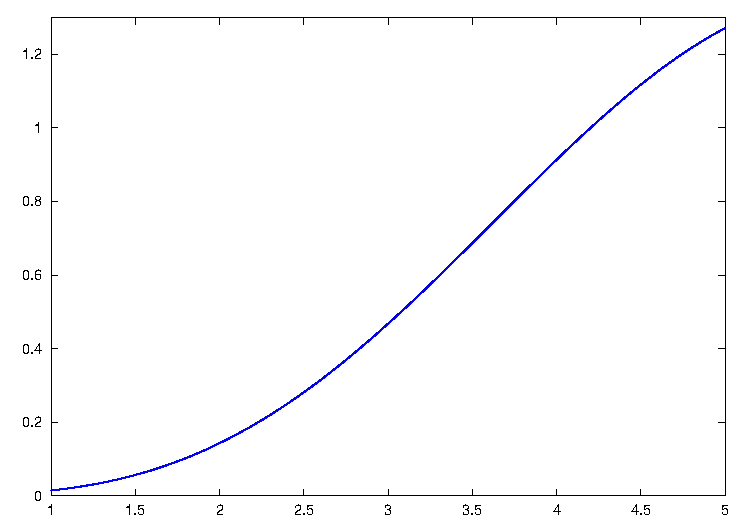
\includegraphics[width=8cm, keepaspectratio]{fig/primera.pdf}
  \end{figure}
\end{frame}


\defverbatim[colored]\testcode{
\begin{lstlisting}
>> 2+2
ans =  4
>> mean([1,2,3,4,5,6,7,8,9])
ans =  5
>> abs(3+4i)
ans =  5
\end{lstlisting}
}

\begin{frame}
  \frametitle{¿Una calculadora programable?}
  \testcode
\end{frame}

\begin{frame}
  \frametitle{Todo esto es muy bonito pero...}
  \begin{itemize}
    \item ¿Es una herramienta realmente útil?
    \item ¿Se usa masivamente en la industria?
    \item ¿Por qué?
    \item ¿Cuánto cuesta Matlab?
    \item ¿Es la única solución?
  \end{itemize}
\end{frame}

\begin{frame}
  \frametitle{Octave}
  \begin{itemize}
    \item Implementación libre y gratuita del lenguaje Matlab
    \item \url{http://www.octave.org}
    \item Programa muy utilizado en GNU/Linux
    \item Versiones para Windows y Mac
    \item QtOctave
    \item \emph{Libre y gratuito}
  \end{itemize}
\end{frame}

\begin{frame}
  \frametitle{El lenguaje Matlab}
  \begin{itemize}
    \item Caracteres especiales
    \item Funciones y scripts
    \item Tipos
    \item Variables
    \item Operadores
    \item Sentencias
    \item Contenendores
      \begin{itemize}
      \item \emph{Function handles}
      \end{itemize}
  \end{itemize}
\end{frame}

\defverbatim[colored]\testcode{
\begin{lstlisting}
>> % Este comando sera ignorado
>> 'hola' % 'Hola,Matlab!'
ans = hola

>> 'hola';
>> 'hola', 'que tal'
ans = hola
ans = que tal

>> 'hola', ...
'que tal'
ans = hola
ans = que tal
\end{lstlisting}
}

\begin{frame}
\frametitle{Caracteres especiales}
\testcode
\end{frame}

\begin{frame}
\frametitle{El directorio de trabajo}
\begin{itemize}
\item Matlab puede ejecutar archivos con código
\item Matlab puede cargar archivos de datos
\item La biblioteca de funciones está formada por archivos con código.
\item Matlab busca en sus directorios de sistema más el \emph{directorio de
  trabajo}
\item Variable \texttt{path}
\end{itemize}
\end{frame}


\defverbatim[colored]\testcode{
\begin{lstlisting}
function [sal1,sal2,...] = nombre(ent1,ent2,...)
  sentencias ejecutables
  sal1 = ...
  sal2 = ...
\end{lstlisting}
}

\begin{frame}
\frametitle{Funciones. Sintaxis}
\testcode

Lo guardaremos todo en \emph{el directorio de trabajo} en un archivo
llamado \emph{nombre.m}
\end{frame}

\begin{frame}
\frametitle{Scripts}
\begin{itemize}
\item Un script es un programa
\item Un programa es una secuencia de instrucciones ejecutables
\item Un programa no depende de variables externas
\item También se guarda en un archivo \emph{.m} en el \emph{directorio
  de trabajo}
\item Se ejecuta escribiendo el nombre del archivo en la consola o
  pulsando \texttt{F5} en el editor.
\end{itemize}
\end{frame}

\defverbatim[colored]\testcode{
\begin{lstlisting}
function y = aprsin(x)
  y=x-(x.^3)/6
\end{lstlisting}
}
\begin{frame}
  \frametitle{Nuestra primera función}
Abrimos un archivo nuevo en el editor
\testcode
Y lo guardamos en el directorio de trabajo como \texttt{aprsin.m}.
\end{frame}

\defverbatim[colored]\testcode{
\begin{lstlisting}
x=linspace(-pi,pi,100);
for i = 1:100
  y(i)=aprsin(x(i));
end
plot(x,[y;sin(x)])
\end{lstlisting}
}

\begin{frame}
\frametitle{Nuestro primer script}
En un archivo nuevo del editor
\testcode
Lo guardamos con el nombre \texttt{comparar.m} \emph{en el directorio
  de trabajo}. Luego pulsamos \texttt{F5}
\end{frame}

\begin{frame}
\frametitle{El resultado}
  \begin{figure}[h]
    \centering{}
    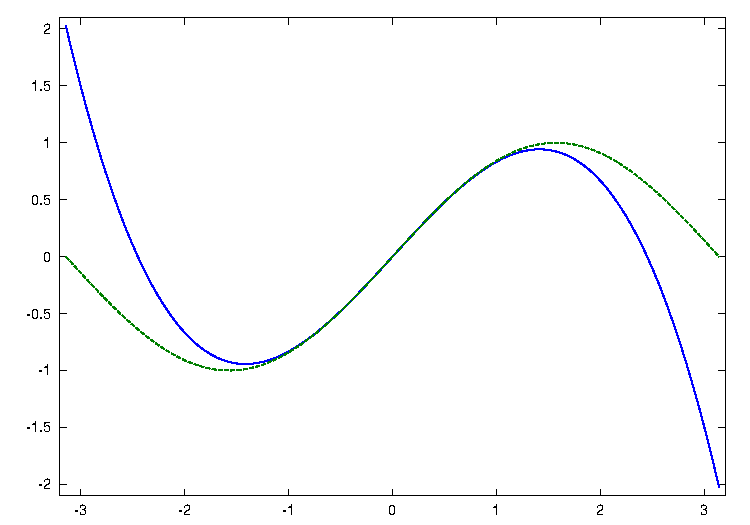
\includegraphics[width=8cm, keepaspectratio]{fig/comparar.pdf}
  \end{figure}
\end{frame}


\defverbatim[colored]\testcode{
\begin{lstlisting}
help eig
\end{lstlisting}
}

\begin{frame}
\frametitle{Ayuda. Función \texttt{help}}
\begin{itemize}
\item En Matlab todo es una función
\item Cada función contiene una pequeña ayuda
\item Para consultar la ayuda existe la función \texttt{help}
\end{itemize}
\testcode
\end{frame}

\begin{frame}
\frametitle{Tipos}
Es importante diferenciar los conceptos de
\begin{description}
  \item[Tipo] Cualquier elemento de un código tiene un tipo:
    caracteres, números, matrices...
  \item[Variable] Identificador asignado a un tipo o a un contenedor
  \item[Argumento] Variable de entrada o salida de una unidad de
    programa
\end{description}
\end{frame}

\begin{frame}
\frametitle{Tipos numéricos}
\begin{itemize}
  \item Tipo por defecto: arrays n-dimensionales de doble precisión
  \item Simple precisión
  \item Enteros de varios bits
\end{itemize}
\end{frame}

\defverbatim[colored]\testcode{
\begin{lstlisting}
>> a = pi
a = 3.1416
>> a(1)
ans = 3.1416
>> a(1,1)
ans = 3.1416
>> a(1,1,1)
ans = 3.1416
\end{lstlisting}
}

\begin{frame}
\frametitle{Mira qué curioso}
\testcode
\end{frame}

\begin{frame}
\frametitle{Escribir matrices}
\begin{itemize}
  \item El espacio o la coma separan elementos de la misma fila
  \item El retorno de carro o el punto y coma separa filas
\end{itemize}
\[ \left(
\begin{array}{ccc}
1&2&3\\
4&5&6\\
7&8&9
\end{array} \right)
\]
\end{frame}


\defverbatim[colored]\testcode{
\begin{lstlisting}
M=[1,2,3;4,5,6;7,8,9];
\end{lstlisting}
}

\begin{frame}
\frametitle{Ejercicio 1}
\testcode
Escribir 
\[ \left(
\begin{array}{ccc}
1&2&3\\
4&5&6\\
7&8&9
\end{array} \right)
\]
de otros 3 modos posibles.
\end{frame}

\begin{frame}
\frametitle{Subíndices}
\begin{itemize}
  \item En Matlab el primer índice cuenta elementos en la columna
  \item El segundo índice cuenta elementos en la fila
  \item \emph{Pero} un vector es siempre fila a no ser que se diga lo
    contrario.
  \item El truco es que no nos preocupen las filas y las columnas,
    sólo los índices
\end{itemize}
\[ M_{ij} = M(i,j) \]
\end{frame}

\defverbatim[colored]\testcode{
\begin{lstlisting}
>> v(4)=2
v =

   0   0   0   2

>> w(4,1)=2
w =

   0
   0
   0
   2
\end{lstlisting}
}
\begin{frame}
\frametitle{No hay quien te entienda}
\testcode
\end{frame}

\defverbatim[colored]\testcode{
\begin{lstlisting}
>> v=[1,2,3,4,5];
>> v(4)
ans = 4
\end{lstlisting}
}

\begin{frame}
\frametitle{Un vector...}
\[v = (1,2,3,\textcolor{red}{4},5) \]
\testcode
\end{frame}

\defverbatim[colored]\testcode{
\begin{lstlisting}
>> M=[1,2,3;4,5,6;7,8,9];
>> M(2,3)
ans =  6
\end{lstlisting}
}

\begin{frame}
\frametitle{Una matriz...}
\[ \left(
\begin{array}{ccc}
1&2&3\\
4&5&\textcolor{red}{6}\\
7&8&9
\end{array} \right)
\]
\testcode
\end{frame}


\defverbatim[colored]\testcode{
\begin{lstlisting}
>> M([1,2],[2,3])
ans =

   2   3
   5   6
\end{lstlisting}
}

\begin{frame}
\frametitle{Podemos indexar con vectores}
\[ \left(
\begin{array}{ccc}
1&\textcolor{red}{2}&\textcolor{red}{3}\\
4&\textcolor{red}{5}&\textcolor{red}{6}\\
7&8&9
\end{array} \right)
\]
\testcode
\end{frame}

\defverbatim[colored]\testcode{
\begin{lstlisting}
>> M(2,:)
ans =

   4   5   6
\end{lstlisting}
}

\begin{frame}
\frametitle{O con índices mudos}
\[ \left(
\begin{array}{ccc}
1&2&3\\
\textcolor{red}{4}&\textcolor{red}{5}&\textcolor{red}{6}\\
7&8&9
\end{array} \right)
\]
\testcode
\end{frame}

\defverbatim[colored]\testcode{
\begin{lstlisting}
\end{lstlisting}
}

\defverbatim[colored]\testcode{
\begin{lstlisting}
>> 0:2:10
ans =
   0   2   4   6   8  10

>> 0:5
ans =
  0  1  2  3  4  5
\end{lstlisting}
}


\begin{frame}
\frametitle{Secuencias}
\begin{itemize}
\item Es una abreviatura común para escribir un vector fila
\item La sintaxis es \texttt{inicio:incremento:final}
\end{itemize}
\testcode
\end{frame}

\begin{frame}
\frametitle{Ejercicio 2} 
Crear la matriz siguiente y extraer de ella la submatriz marcada en rojo.
\[ \left( \begin{array}{ccccc}
11&12&13&14&15\\
21&22&23&24&25\\
31&32&\textcolor{red}{33}&\textcolor{red}{34}&\textcolor{red}{35}\\
41&42&\textcolor{red}{43}&\textcolor{red}{44}&\textcolor{red}{45}\\
51&52&\textcolor{red}{53}&\textcolor{red}{54}&\textcolor{red}{55}
\end{array} \right) \]
\end{frame}

\begin{frame}
\frametitle{Otros tipos}
\begin{itemize}
\item La unidad imaginaria es \emph{i}, \emph{j}, \emph{I} o \emph{J}
\item Las cadenas de texto se introducen entre comillas simples
\item Los tipos lógicos son \emph{true} y \emph{false}.  \emph{true}
  es $\not \equiv 0$ y \emph{false} es $\equiv 0$
\end{itemize}
\end{frame}

\begin{frame}
\frametitle{Operadores}
\begin{itemize}
\item Operadores matriciales \texttt{+}, \texttt{-}, \texttt{*},
  \texttt{/}, \texttt{\^}
\item Operadores escalares \texttt{.*}, \texttt{./}, \texttt{.\^}
\item Operadores lógios matriciales \texttt{\&}, \texttt{|}, \texttt{!}
\item Relaciones de comparación \texttt{<}, \texttt{>}, \texttt{==},
  \texttt{<=}, \texttt{>=}, \texttt{!=}
\item Relaciones lógicas \texttt{\&\&}, \texttt{||}
\end{itemize}
\end{frame}

\defverbatim[colored]\testcode{
\begin{lstlisting}
>> a=rand(3,3);
>> a=rand(3,3);b=rand(3,3);
>> a*b
ans =
    1.0297    0.9105    0.3293
    0.9663    0.8267    0.4211
    0.5355    0.4318    0.3279
>> a.*b
ans =
    0.1824    0.3253    0.0563
    0.5500    0.6003    0.1897
    0.0458    0.0017    0.1822
\end{lstlisting}
}

\begin{frame}
\frametitle{El error más común de Matlab}
\testcode
\end{frame}

\defverbatim[colored]\testcode{
\begin{lstlisting}
>> a=[1,2,3;4,5,6;7,8,9];
>> a.^pi
ans =
    1.0000    8.8250   31.5443
   77.8802  156.9925  278.3776
  451.8079  687.2913  995.0416
>> a^pi
ans =
 1.0e+03 *
 0.69 - 0.0004i 0.85 - 0.0001i 1.01 + 0.0002i
 1.57 - 0.0000i 1.93 - 0.0000i 2.29 + 0.0000i
 2.45 + 0.0003i 3.01 + 0.0001i 3.57 - 0.0002i
\end{lstlisting}
}

\begin{frame}
\frametitle{El error más común de Matlab}
\testcode
\end{frame}

\begin{frame}
\frametitle{Ejercicio 3}
\end{frame}

\begin{frame}
\frametitle{Control de flujo}
\begin{itemize}
\item Las sentencias son palabras clave necesarias para programar
\item Son comunes a la mayoría de lenguajes de programación
\item Control de flujo es el uso de bucles, condicionales, casos...
\item El control de flujo implica el encapsulamiento de una tarea.
\end{itemize}
\end{frame}

\defverbatim[colored]\testcode{
\begin{lstlisting}
if cond
  sentencias
elseif cond
  sentencias
else
  sentencias
end
\end{lstlisting}
}

\begin{frame}
\frametitle{Condicionales o \texttt{if}}
\testcode
\end{frame}

\defverbatim[colored]\testcode{
\begin{lstlisting}
for var=contador
  sentencias
end
\end{lstlisting}
}

\begin{frame}
\frametitle{Bucles o \texttt{for}}
\testcode
\begin{itemize}
\item \texttt{contador} puede ser un vector o una secuencia
\item Para cada paso \texttt{i} avanza de valor en \texttt{contador}
\item Las sentencias pueden depender o no de \texttt{i}
\end{itemize}
\end{frame}


\begin{frame}
\frametitle{Más control de flujo}
\begin{description}
\item[case] Control de casos finitos
\item[while] Bucle controlado por condición lógica
\item[try] Control de excepciones
\item[break] Salida de bloques
\item[continue] Idem
\item[return] vuelta al programa principal
\end{description}
\end{frame}

\begin{frame}
\frametitle{Ejercicio 4}
\end{frame}

\begin{frame}
\frametitle{Contenedores}
\begin{itemize}
\item Estructuras de datos. Forma de árbol
\item Cell arrays. Forma de matriz
\item Function handles. Contenedor para una función.
\begin{itemize}
  \item Funciones anónimas
\end{itemize}
\end{itemize}
\end{frame}


\defverbatim[colored]\testcode{
\begin{lstlisting}
>> ed.num=1.234;
>> ed.str='hola';
>> ed.logic.true=1;
>> ed.logic.false=0;
>> ed

ed =

      str: 'hola'
      num: 1.2340
    logic: [1x1 struct]
\end{lstlisting}
}

\begin{frame}
\frametitle{Estructuras de datos}
\testcode
\end{frame}

\defverbatim[colored]\testcode{
\begin{lstlisting}
>> celda={1.234,'hola';true,false}
celda =
  [1.2340]    'hola'
  [     1]    [   0]

>> celda{1,1}
ans =  1.2340
\end{lstlisting}
}

\begin{frame}
\frametitle{Cell arrays}
\testcode
\end{frame}

\defverbatim[colored]\testcode{
\begin{lstlisting}
>> fhsin = @sin
fhsin =

    @sin

>> fhsin(pi/2)
ans =  1
\end{lstlisting}
}

\begin{frame}
\frametitle{Function Handles}
Es capaz de contener una función.
\testcode
\end{frame}

\begin{frame}
\frametitle{Ejercicio 5}
\end{frame}


\defverbatim[colored]\testcode{
\begin{lstlisting}
>> test1 = @(x) x.*sin(x)
test1 =
@(x) x .* sin (x)
>> test1(1)
ans =  0.84147

>> test2 = @(x,y) exp(-(x.^2+y.^2))
test2 =
@(x, y) exp (-(x .^ 2 + y .^ 2))
>> test2(1,i)
ans =  1
\end{lstlisting}
}

\begin{frame}
\frametitle{Funciones anónimas} 
Permiten crear un \emph{function handle} definiendo la función
directamente.
\testcode
\end{frame}

\begin{frame}
\frametitle{Conclusiones}
\begin{itemize}
\item El lenguaje Matlab es muy limitado
\item Es sencilloy su sintaxis es clara
\item Sus estructuras son muy matemáticas
\item Está basdo en funcionesy no conocemos ninguna
\item La biblioteca de funciones de Matlab es tan grande como quieras
  pagarla.
\end{itemize}
\end{frame}

\begin{frame}
\frametitle{Creación de matrices}
\begin{description}
\item[eye] matriz de ceros con unos en la diagonal
\item[linspace] Vector de elementos equiespaciados
\item[logspace] Vector de elementos con el exponente equiespaciado
\item[meshgrid] Matrices de elementos equiespaciados en 2D
\item[ones] Matriz de unos
\item[zeros] Matriz de ceros
\item[rand] Matriz de números aleatorios
\end{description}
\end{frame}

\begin{frame}
\frametitle{Manipulación de matrices}
\begin{description}
\item[reshape] Cambia la forma de la matriz conservando el número de
  elementos
\item[transpose] Traspuesta. Equivale a .'
\item[ctranspose] Matriz conjugada. Equivale a '
\item[rot90] Gira la matriz 90 grados hacia la izquierda
\end{description}
\end{frame}

\begin{frame}
\frametitle{Ejercicio 6}
\end{frame}

\defverbatim[colored]\testcode{
\begin{lstlisting}
>> A=[1,0;2,1];y=[2;4];
>> x=A\y
x =

  2
  0
\end{lstlisting}
}

\begin{frame}
\frametitle{Resolución de SEL}

Para resolver sistemas de ecuaciones lineales contamos con un operador
universal
\testcode
\end{frame}

\begin{frame}
\frametitle{Cálculo Simbólico}
\begin{itemize}
\item Podéis hacer operaciones simbólicas con Matlab
\pause
\item Que pueda hacerse no significa que tenga que hacerse
\pause
\item También podéis depilaros las cejas con una sierra mecánica
\end{itemize}
\end{frame}

\begin{frame}
\frametitle{Integración numérica}
\begin{description}
\item[quad] Integración numérica. 3 argumentos de entrada
\item[quadl] Algoritmo de integración mejorado
\item[dblquad] Integración bidimensional de funciones de dos variables
\item[trapz] Regla del trapecio
\end{description}
\end{frame}

\begin{frame}
\frametitle{Ejercicio 7}
\end{frame}

\defverbatim[colored]\testcode{
\begin{lstlisting}
>> p = [1 1 0];
>> polyval(p,1)
ans =  2
>> roots(p)
ans =
  -1
   0
\end{lstlisting}
}

\begin{frame}
\frametitle{Desarrollos en serie de funciones}
\begin{itemize}
\item Los coeficientes de un desarrollo en serie son un vector
\end{itemize}
$x^2 + x$ es $1x^2+1x+0$, es decir [1 1 0]
\testcode
\end{frame}

\begin{frame}
\frametitle{Polinomios}
\begin{description}
\item[polyval] Obtiene el valor en un punto
\item[roots] Obtiene las raíces del polinomio
\item[polyder] Deriva un polinomio
\item[polyinteg] Integra un polinomio
\item[conv] Multiplica dos polinomios
\item[residue] Desarrollo en fracciones parciales.
\end{description}
\end{frame}

\begin{frame}
\frametitle{Funciones que devuelven polinomios}
\begin{description}
\item[poly] Obtiene el polinomio característico de una matriz.
\item[polyfit] Modelo polinómico de una serie de datos.
\end{description}
\end{frame}

\begin{frame}
\frametitle{Representación gráfica}
\begin{itemize}
\item Representar datos es sencillo e intuitivo
\item No hay que emocionarse con la representación gráfica
\item Sólo veremos curvas en el plano
\item ¿Necesitamos más?
\end{itemize}
\end{frame}

\defverbatim[colored]\testcode{
\begin{lstlisting}
>> x=linspace(0,500,100000);
>> plot(x,exp(-x/100).*sin(x))
\end{lstlisting}
}

\begin{frame}
\frametitle{Plot}
Representa curvas en el plano. $e^{-x/100}\sin x$ para $x\in[0,500]$
\testcode
\end{frame}

\begin{frame}
\frametitle{El resultado}
  \begin{figure}[h]
    \centering{}
    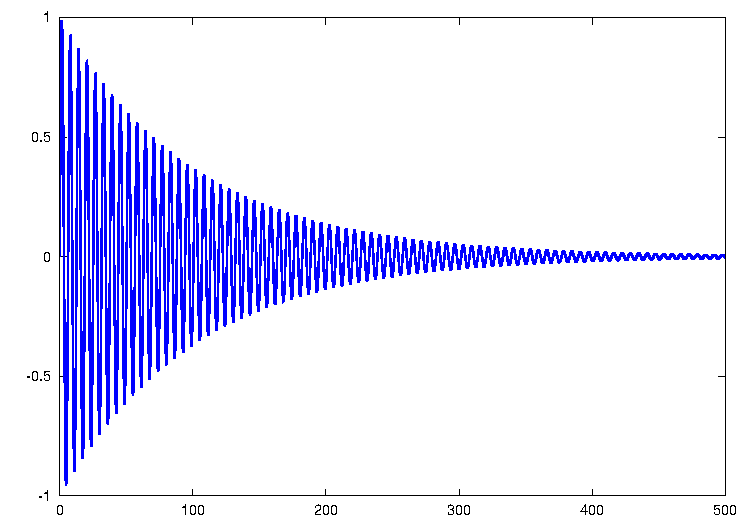
\includegraphics[width=8cm, keepaspectratio]{fig/abanico.pdf}
  \end{figure}
\end{frame}

\defverbatim[colored]\testcode{
\begin{lstlisting}
>> title('Una funcion cualquiera')
>> xlabel('Tiempo')
>> ylabel('Amplitud')
\end{lstlisting}
}

\begin{frame}
\frametitle{Etiquetas}
\testcode
\end{frame}

\begin{frame}
\frametitle{El resultado}
  \begin{figure}[h]
    \centering{}
    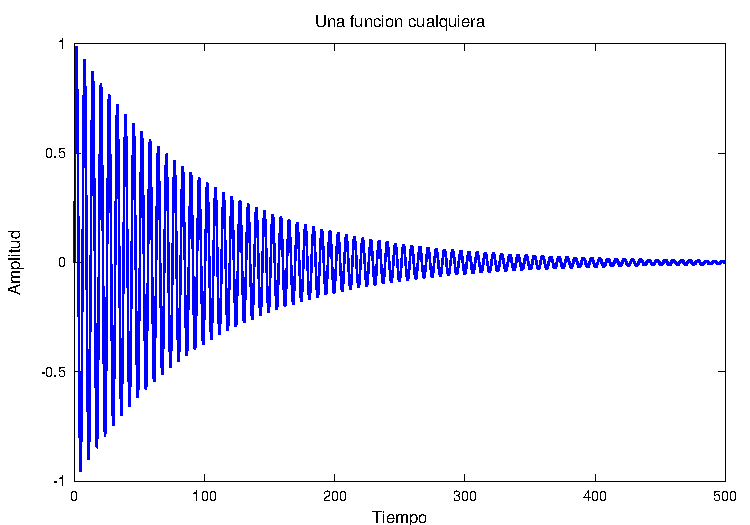
\includegraphics[width=8cm, keepaspectratio]{fig/abanico2.pdf}
  \end{figure}
\end{frame}

\defverbatim[colored]\testcode{
\begin{lstlisting}
>> x=linspace(-pi,pi,100);
>> plot(x,sin(x),'m:',...
x,cos(x),'k^',x,tan(x),'bx')
>> axis([-pi,pi,-2,2])
>> grid on
>> legend('linea de puntos magenta',...
          'triangulos negros',...
          'cruces azules') 
\end{lstlisting}
}
\begin{frame}
\frametitle{Estilos}
\testcode
\end{frame}

\begin{frame}
\frametitle{El resultado}
  \begin{figure}[h]
    \centering{}
    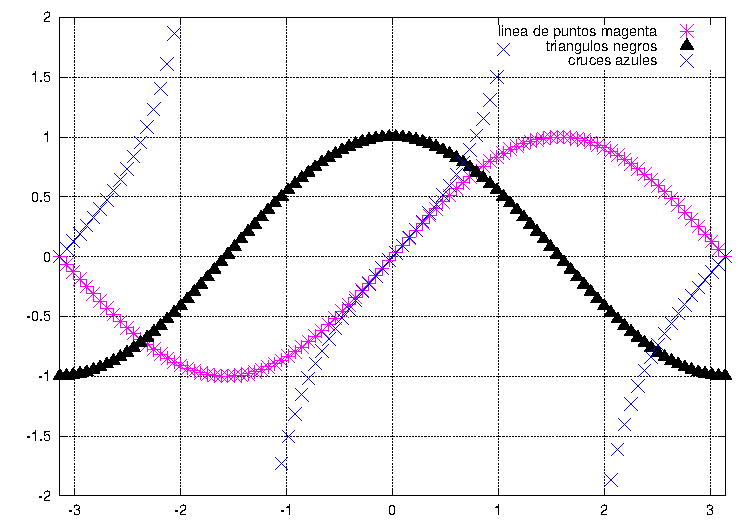
\includegraphics[width=8cm, keepaspectratio]{fig/trigplot.pdf}
  \end{figure}
\end{frame}

\begin{frame}
\frametitle{hold}
\begin{itemize}
\item La ventana gráfica se borra automáticamente cada vez que
  dibujamos algo
\item Para cambiar el comportamiento anterior se usa la función
  \emph{hold}
  \begin{itemize}
    \item \texttt{hold on} mantiene todo lo dibujado en la pantalla
    \item \texttt{hold off} vuelve al comportamiento inicial
  \end{itemize}
  \item Para borrar la ventana gráfica usamos \texttt{clf}
\end{itemize}
\end{frame}

\begin{frame}
\frametitle{\texttt{figure}}
\begin{itemize}
\item Las ventanas gráficas se manipulan con la función
  \texttt{figure}
\item Cada ventana gráfica tiene asociada un número entero
  \begin{itemize}
    \item \texttt{figure} se llama con un número que corresponde al de
      la ventana
    \item Si utilizamos un número que no corresponde a ninguna ventana
      existente crearemos una nueva con este número asociado
    \item Si utilizamos un número existente activaremos la ventana
      correspondiente
  \end{itemize}
\end{itemize}
\end{frame}

\defverbatim[colored]\testcode{
\begin{lstlisting}
>> x= linspace(-pi,pi,100);
>> subplot(2,2,1)
>> plot(x,sin(x))
\end{lstlisting}
}
\begin{frame}
  \frametitle{subplot}
  Es el comando que permite poner varios ejes en una misma figura
\testcode
Primero de los cuatro sectores.
\end{frame}

\begin{frame}
\frametitle{El resultado}
  \begin{figure}[h]
    \centering{}
    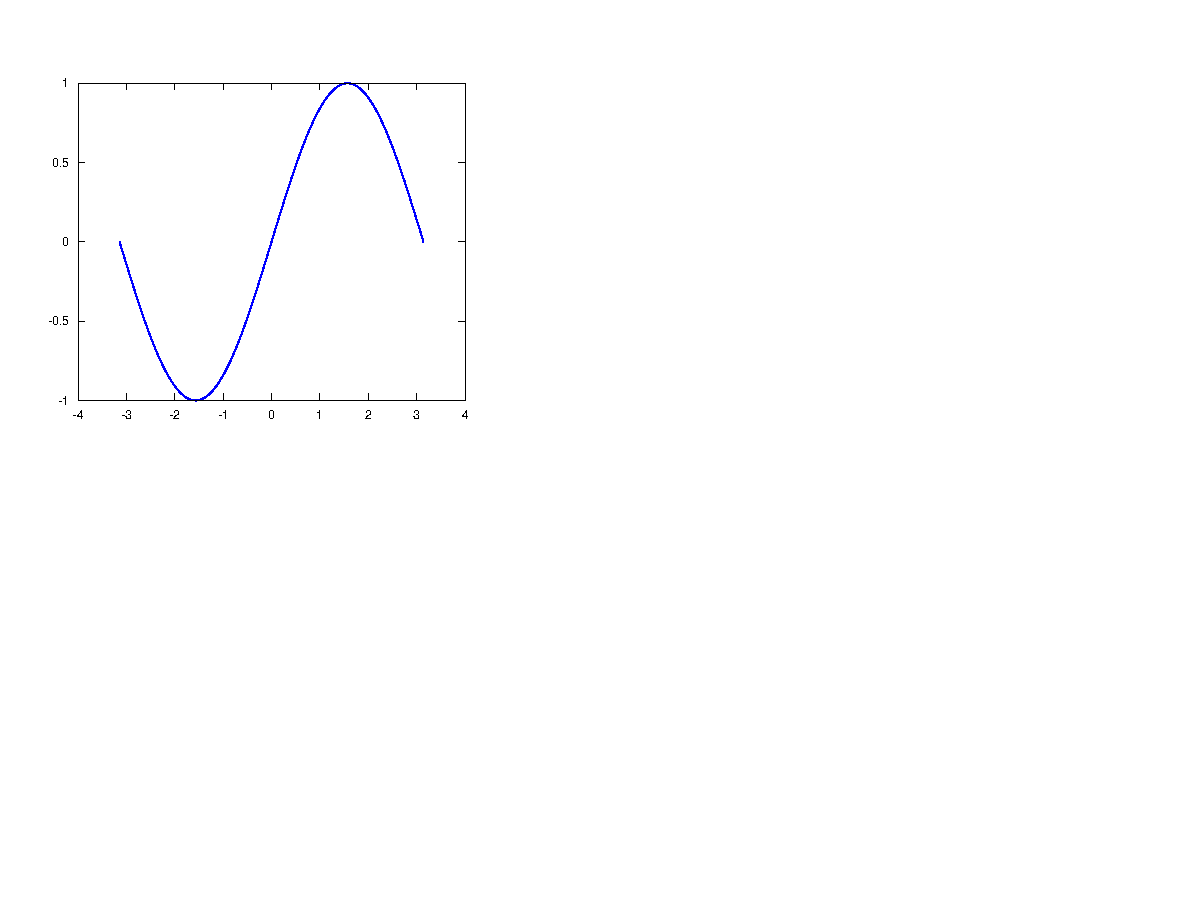
\includegraphics[width=8cm, keepaspectratio]{fig/subplot1.pdf}
  \end{figure}
\end{frame}


\defverbatim[colored]\testcode{
\begin{lstlisting}
>> subplot(2,2,2)
>> plot(x,cos(x))
>> subplot(2,2,3)
>> plot(x,sinh(x))
>> subplot(2,2,4)
>> plot(x,cosh(x))
\end{lstlisting}
}

\begin{frame}
\frametitle{subplot}
Ahora completamos los cuatro cuadrantes.
\testcode
\end{frame}

\begin{frame}
\frametitle{El resultado}
  \begin{figure}[h]
    \centering{}
    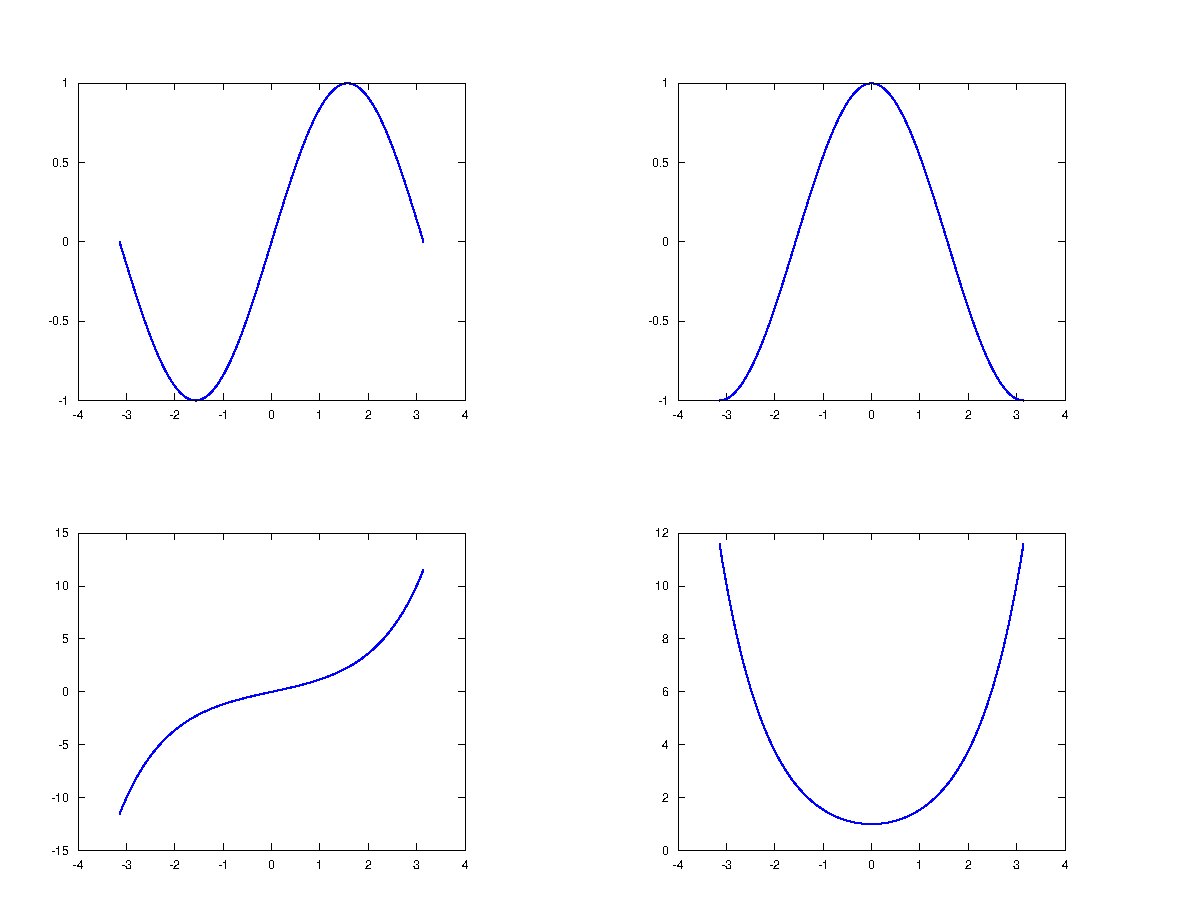
\includegraphics[width=8cm, keepaspectratio]{fig/subplot2.pdf}
  \end{figure}
\end{frame}

\begin{frame}
\frametitle{Otros comandos}
\begin{description}
\item[semilogx] Dibuja una curva con el eje x en escala logarítmica
\item[semilogy] Dibuja una curva con el eje y en escala logarítmica
\item[loglog] Dibuja una curva en escala logarítmica
\end{description}
\end{frame}

\begin{frame}
\frametitle{Ejercicio 8}

Representar en una misma ventana y dos frames (uno superior y otro
inferior) la función

\[ \sqrt{x} \sin(1/x)\ \ x \in[0.001,1]  \]

en escala normal y en escala semilogarítmica en el eje x.
\end{frame}

\begin{frame}
\frametitle{Comandos interesantes}
\begin{description}
\item[\texttt{get}, \texttt{set}] Cambia los atributos de un plot
  handle
\item[\texttt{text}] Pone texto en la figura
\item[\texttt{contour}] Isolíneas de una matriz de datos en 3D
\item[\texttt{griddata}] Interpola para el contour
\end{description}
\end{frame}

\begin{frame}
\frametitle{Desarrollos de datos}
\begin{description}
\item[\texttt{interp1}] Interpolación de una serie de puntos
\item[\texttt{interp2}] Interpolación de una nube de puntos
\item[\texttt{polyfit}] Coeficientes del polinomio de grado \emph{n}
  con mínimo error cuadrático
\item[\texttt{fft}] Realiza la transformada de Fourier
\end{description}
\end{frame}

\defverbatim[colored]\testcode{
\begin{lstlisting}
>> x=[1 2 3 4 5 6 7 8];
>> y=[1 4 2 5 7 4 2 7];
>> interp1(x,y,7.234,'spline')
ans = 2.3437
>> test=@(x,y,z) interp1(x,y,z,'spline');
>> test(x,y,7.234)
ans = 2.3437
\end{lstlisting}
}


\begin{frame}
\frametitle{\texttt{interp1}}
\testcode
\end{frame}

\defverbatim[colored]\testcode{
\begin{lstlisting}
>> x=[1 2 3 4 5 6 7 8];
>> y=[2 4 3 5 6 5 7 9];
>> coeff=polyfit(x,y,3);
>> plot(x,y,'k+',1:0.1:8,...
polyval(coeff,1:0.1:8),'b-')
\end{lstlisting}
}

\begin{frame}
\frametitle{\texttt{polyfit}}
\testcode
\end{frame}

\begin{frame}
\frametitle{El resultado}
  \begin{figure}[h]
    \centering{}
    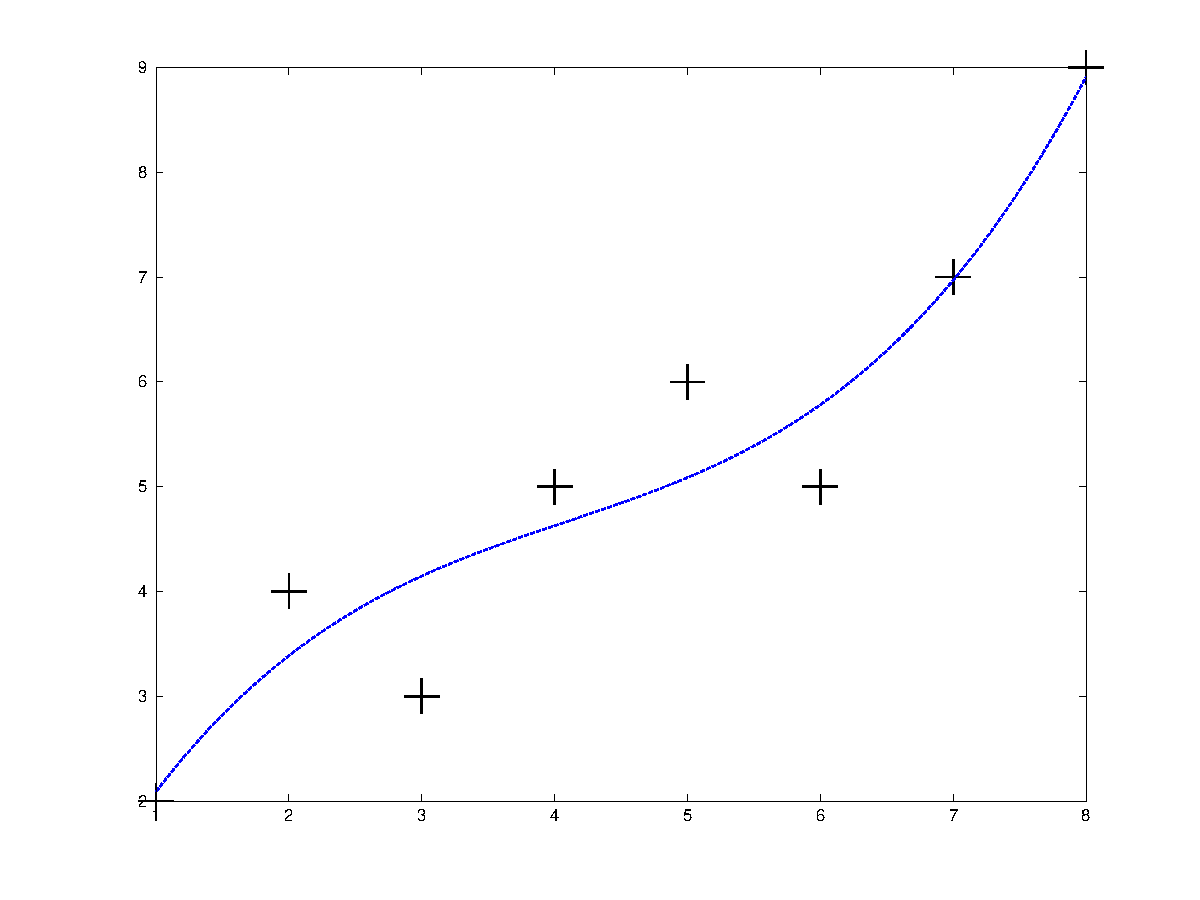
\includegraphics[width=8cm, keepaspectratio]{fig/polyfit.pdf}
  \end{figure}
\end{frame}

\begin{frame}
\frametitle{Estadística descriptiva}
\begin{description}
\item[\texttt{mean}] Media
\item[\texttt{std}] Desviación típica
\item[\texttt{median}] Mediana
\item[\texttt{sort}] Orena los elementos de menor a mayor
\item[\texttt{center}] Elimina la media de una muestra
\end{description}
\end{frame}

\begin{frame}
\frametitle{EDO}
\begin{itemize}
\item Es una de las aplicaciones más importantes del Cálculo Numérico
\item Los problemas más comunes son los problemas de Cauchy no lineales
\item En ese caso la solución numérica es esencial
\item Lo más importante es saber si nuestro problema es stiff
\end{itemize}
\end{frame}

\begin{frame}
\frametitle{Stiff}
\begin{itemize}
\item Un problema es \emph{stiff} cuando el paso temporal viene
  determinado por la estabilidad del esquema.
\item Suelen relacionarse con problemas no lineales o condiciones de
  contorno muy exigentes
\item Requieren esquemas de integración temporal implícitos
\end{itemize}
\end{frame}

\begin{frame}
  \frametitle{Funciones}
  \begin{description}
  \item[\texttt{ode45}] Runge-Kutta de paso variable orden 4-5
  \item[\texttt{ode113}] Adams multipaso
  \item[\texttt{ode23s}] Esquema implícito Rosenbrock
  \item[\texttt{lsode}] Octave
  \end{description}
\end{frame}

\begin{frame}
  \frametitle{Van der Pol}
Un caso típico es la ecuación de Van der Pol

\[ x'' + x +\mu(x'^2-1)x = 0 \]

Dependiendo del valor de $\mu$ el problema va a ser \emph{stiff} o no.
\end{frame}

\defverbatim[colored]\testcode{
\begin{lstlisting}
>> [tout,xout]=ode45(@vdp1,[0 20],[2 0])
>> plot(tout,xout(:,1))
\end{lstlisting}
}

\begin{frame}\frametitle{Solución}
\testcode
\end{frame}


\begin{frame}
  \frametitle{Solución}
  \begin{figure}[h]
    \centering{}
    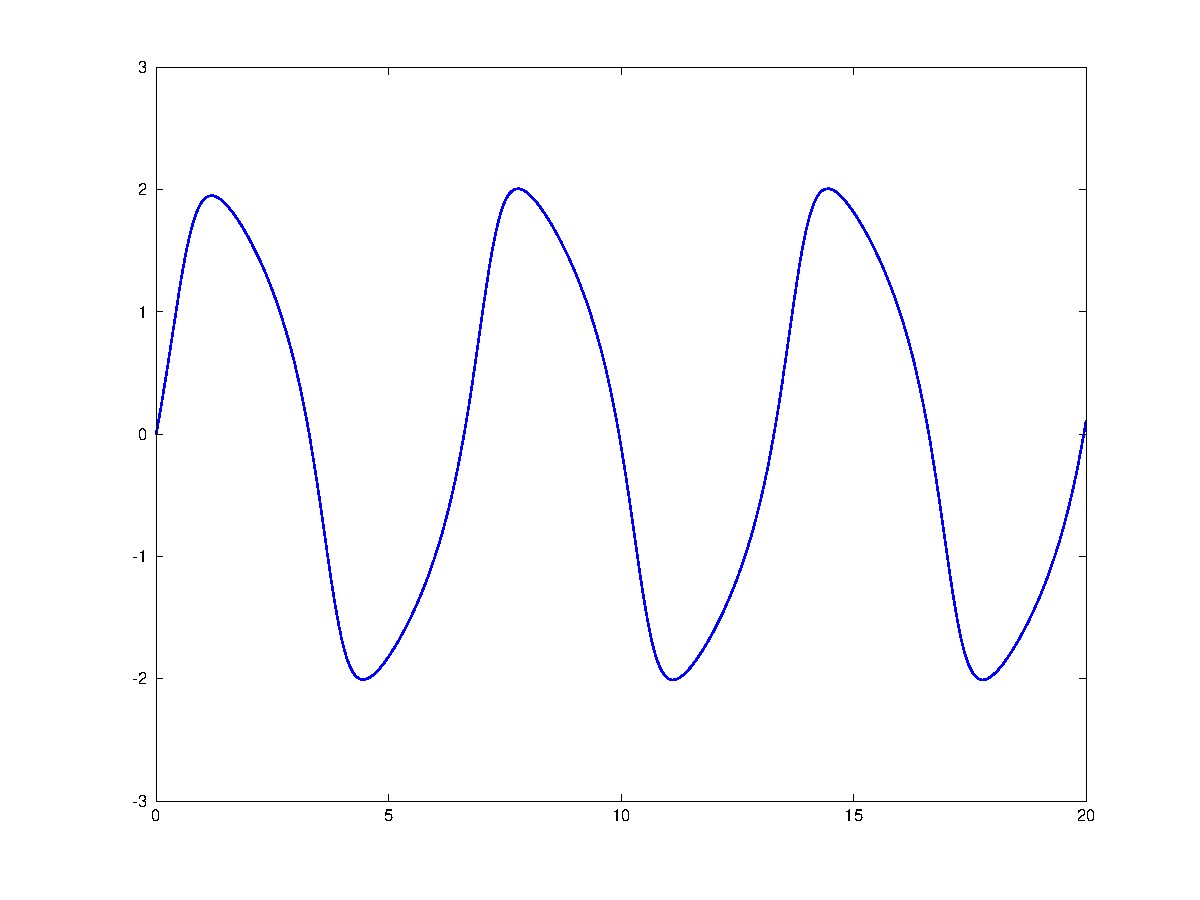
\includegraphics[width=8cm, keepaspectratio]{fig/vdp1.pdf}
  \end{figure}
\end{frame}

\defverbatim[colored]\testcode{
\begin{lstlisting}
>> [tout,xout]=ode23s(@vdp1000,[0 20],[2 0])
>> plot(tout,xout(:,1))
\end{lstlisting}
}

\begin{frame}\frametitle{Solución}
\testcode
\end{frame}


\begin{frame}
  \frametitle{Solución}
  \begin{figure}[h]
    \centering{}
    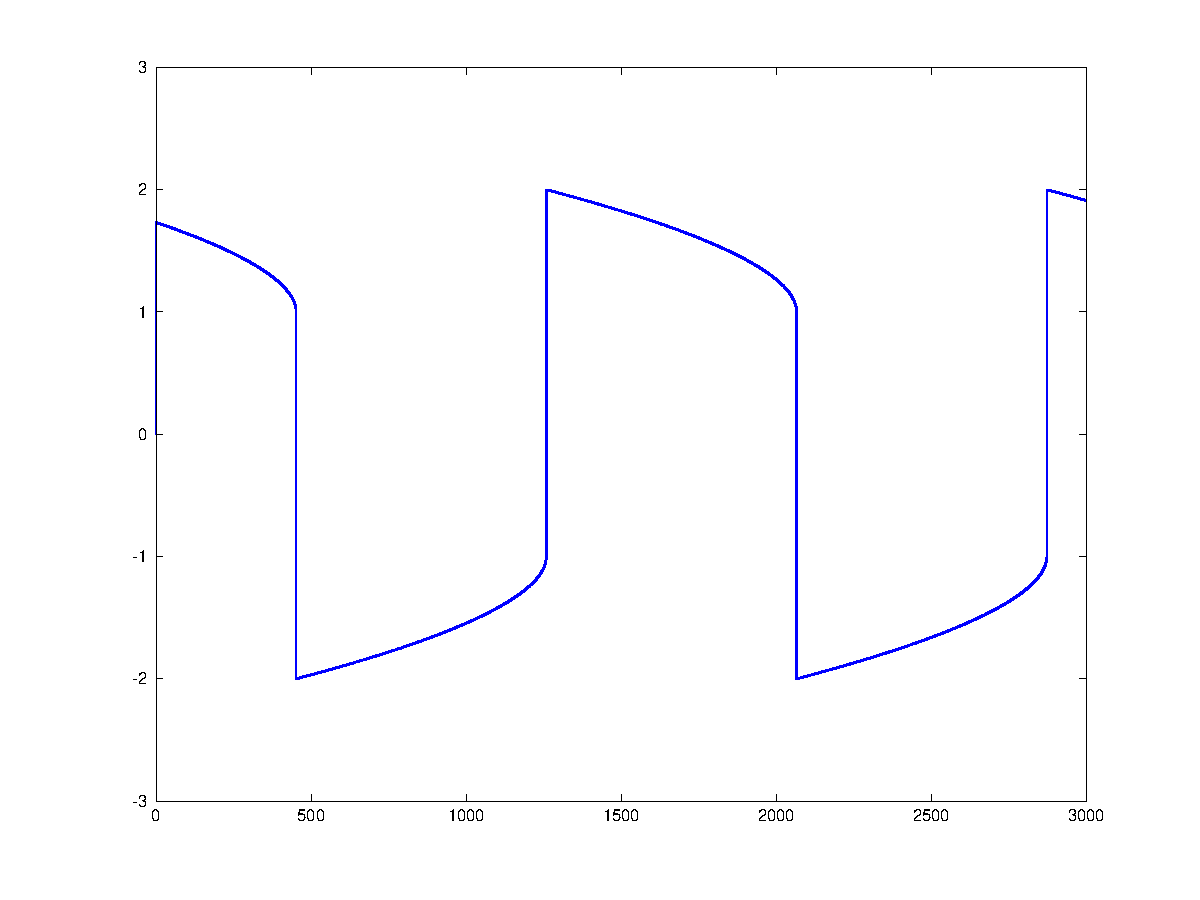
\includegraphics[width=8cm, keepaspectratio]{fig/vdp1000.pdf}
  \end{figure}
\end{frame}

\begin{frame}
  \frametitle{Ejercicio 9}
\end{frame}

\end{large}
\end{document}
